%\documentclass[10pt,conference]{IEEEtran}
\documentclass[sigconf,review]{acmart}
% The preceding line is only needed to identify funding in the first footnote. If that is unneeded, please comment it out.
%\usepackage{cite}
\usepackage{amsmath,amssymb,amsfonts}
%\usepackage{algorithmic}
\usepackage{graphicx}
\usepackage{textcomp}
\usepackage{xcolor}
\usepackage{url}
\usepackage{booktabs}
\usepackage{xspace}
\usepackage{enumitem}
\def\BibTeX{{\rm B\kern-.05em{\sc i\kern-.025em b}\kern-.08em
    T\kern-.1667em\lower.7ex\hbox{E}\kern-.125emX}}

\newcommand{\subheading}[1]{\vspace{1mm} \noindent {\bf #1}}

\definecolor{ScarletRed}{rgb}{0.80,0.00,0.00}

\newif\ifdraft
\drafttrue

\ifdraft
	\marginparwidth=1.3cm
	\marginparsep=5pt
	\newcommand\remark[1]{%
		\mymarginpar{\raggedright\hbadness=10000\tiny\it #1\par}}
	% TODO marker
	\newcommand{\TODO}[1]{\textbf{\textcolor{ScarletRed}{[TODO: #1]}}\xspace}
\else
	\newcommand\remark[1]	{}
	\newcommand{\TODO}[1]{}
\fi

\begin{document}
\title{Search-Based Software Testing (SBST) \\ ICSE 2020 Workshop Proposal}


\author{Jos\'e Miguel Rojas}
\affiliation{%
  \institution{School of Informatics, University of Leicester}
  \city{Leicester}
  \country{United Kingdom}}
\email{j.rojas@leicester.ac.uk}

\author{Erik M. Fredericks}
\affiliation{%
  \institution{Dept. of Computer Science \& Engineering, Oakland University}
  \city{Rochester, MI}
  \country{USA}}
\email{fredericks@oakland.edu}

\begin{abstract}
  There is a growing realization that optimization techniques can be
  applied to many aspects of the software development process: a
  research area known as Search-Based Software Engineering
  (SBSE). Search-Based Software Testing -- one of the largest research
  areas within SBSE -- is the process of using search-based
  optimization algorithms to specifically address problems in software
  testing. SBST has been applied to a wide variety of testing goals
  including structural, functional, non-functional and state-based
  properties. Many approaches to testing and a wide diverse range of
  development domains have been addressed, including exceptions,
  interactions, integration, mutation, regression, and web
  applications.

  Work in SBST has developed to the point at which it is now ripe for
  combination with other areas of software engineering. The common
  ``lingua franca'' that makes these combinations possible is the
  definition of the fitness function that guides a search algorithm. A
  fitness function is merely a form of a metric, and metrics exist
  across the entire software engineering spectrum. Therefore, the
  central objective of this workshop is to bring together researchers
  and industrial practitioners from SBST and the wider software
  engineering community to share experience and provide directions for
  future research, and to encourage the use of search techniques to
  combine aspects of testing with other aspects of the software
  engineering lifecycle.

  SBST is a one-day workshop aimed at bringing testing researchers
  together with the broader software engineering community to discuss
  state-of-the-art work and set new research directions.
\end{abstract}

%\begin{IEEEkeywords}
%component, formatting, style, styling, insert
%\end{IEEEkeywords}


\maketitle

% \section{Thoughts}

% \begin{itemize}
% \item Theme?  SBST 
% \item Award?
% \item Fishbowl session
% \end{itemize}

\section{Contact Information}

\noindent \textbf{Jos\'e Miguel Rojas}. Address:
School of Informatics, University of Leicester, University Road,
LE1 7RH, Leicester, United Kingdom. Phone: +44 (0) 116 252
3828. Email: \url{j.rojas@leicester.ac.uk}.\\
\textbf{Erik M. Fredericks (main contact person)}. Address:
Department of Computer Science and Engineering, Oakland University, 115 Library Dr.,
Rochester, MI, USA, 48309. Phone: +1 (248) 370 4075
3828. Email: \url{fredericks@oakland.edu}.

\section{Motivation and Objectives}
\label{sec:themes}
  
Search-Based~Software~Engineering (SBSE) \cite{mhbj:manifesto} is
receiving increasing attention from the SE community thanks to the
growing realization that optimization can be applied to many aspects
of the software development process.  Search-Based Software
Testing---the process of using search-based optimization algorithms to
specifically address problems in software testing
\cite{mcminn:survey}---is one of the largest research areas within
SBSE. The potential of SBST to be applied to a vast number of open
complex testing problems (e.g., autonomous driving
functions~\cite{Abdessalem2018}) is increasingly evident. Furthermore,
the recent industrial-scale impact of the Sapienz tool~\cite{Sapienz}
at Facebook showcases the capabilities and potential
of SBST and helps as motivation for the community to continue to work
on SBST techniques and tools.

\noindent Some of the specific topics to be explored in the workshop
include:
	
\subheading{Multi-Objective Solutions.}  SBST can use many fitness
functions at once, presenting the end-user with a choice of
non-dominating solutions at the so-called ``Pareto Front''.
Multi-objective optimization may be used to produce test suites that
aim to satisfy multiple goals, such as generating test suites that
focus on verifying properties as well as covering all of the branches
of a program~\cite{Gay14:risks}.

\subheading{Search-Based Optimization and the Test Oracle.} One of the
most difficult challenges in software testing is the development or
synthesis of the test oracle---an automated judgment of the behavior
of the software~\cite{Harman13:oraclesurvey}.  Search techniques have
the potential to be used in automatic oracle generation, oracle
debugging, and the generation of tests engineered to surface faults
tuned to specific oracles.

\subheading{SBST for Web and Mobile Software.} With the rapid rise of
mobile and web-based software, the need has also emerged for effective
testing of those systems. Search-based techniques have the potential
to make a large impact in these areas, and have been used to---for
example---provide security testing of web
applications~\cite{Thome14:sec}.

\subheading{Human Aspects and Integration into Real Test
  Environments.}  Search-based techniques present the possibility to
take into account domain knowledge or optimize tests for human usage
(for example, incorporating a language model to produce test strings
that aid comprehension \cite{Afshan2013}).

\subheading{Enriching SBST with Machine Learning.} Machine learning
techniques have proven their worth across many aspects of software
development. The use of machine learning to enrich heuristic
optimization algorithms---and the use of search-based techniques to
enhance learning algorithms---may be of incredible benefit to the SBST
community~\cite{Malhotra14:SBT}.

\subheading{Application of SBST in Industrial Practice and the
  Classroom.}  We have begun to see the adoption of SBST techniques in
industrial settings. We would like to explore where SBST can and
should be making an impact.  Similarly, we would like to explore the
practicality of teaching SBST as part of the software engineering or
computer science curriculum.

\subheading{Synergies of SBST and other SE areas.} SBST is also ripe
for combination with other areas of software engineering, e.g.,
requirements optimization and project
planning. %\cite{yyetal:refsq08}.
Possibilities exist to optimize the selection of requirements based
not only on traditional aspects of SBSE for requirements (customer
satisfaction, cost, etc.), but also on the implications for regression
testing (code coverage, test execution time, and test effectiveness).

\subsection{Relevance to Software Engineering}
\label{sec:relevance-se}

SBST has been applied to a wide variety of testing goals including
structural \cite{tonella:classes}, functional \cite{wegener:parking},
non-functional \cite{wegener:verifying} and state-based properties
\cite{joshmh:gecco11}.  Many approaches to testing and a wide diverse
range of development domains have been addressed, including exceptions
\cite{tracey-00}, interactions \cite{cohen:constructing},
% integration \cite{briand:using},
mutation \cite{zhan:search-based}, regression \cite{syetal:issta09},
stress \cite{briand-stress-small} and web applications
\cite{Thome14:sec}. In SBST, the primary concern is to define a
fitness function (or set of fitness functions) that capture the test
objectives.  The fitness function is used to guide a search-based
optimization algorithm, which searches the space of test inputs to
find those that meet the test objectives.  Because any test objective
can, in principle, be re-cast as a fitness function, the approach is
widely applicable---as demonstrated by the prior list of testing
applications.  It is therefore highly relevant to Software
Engineering.  This relevance is further testified by the increasing
cumulative number of publications in the area in the last decade, as
Figure \ref{fig:pubs} shows, providing evidence that SBST is a growing
area~\cite{yzmham:sbse-repository}.

\begin{figure}
\centering
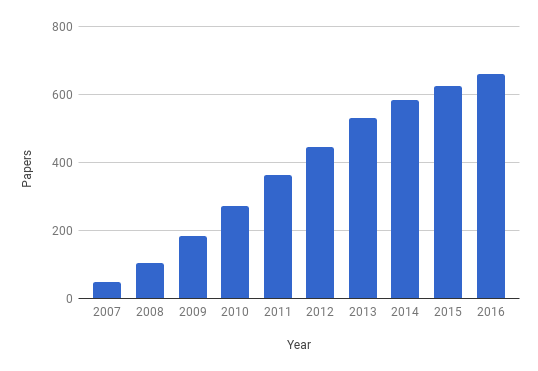
\includegraphics[width=.7\columnwidth]{chart.png}
\caption{\label{fig:pubs}Total number of papers in SBST (2007--2017).}
\end{figure}


\subsection{Relevance To ICSE}
\label{sec:relevance-icse}

The SBST workshop compliments ICSE well. The success of the previous
five editions of SBST which were co-located with ICSE reassures us
that the ICSE community is highly interested in computational search,
and its applications in testing, verification, and a number of other
Software Engineering tasks, and that the key to strenthening and
expanding this exciting research area is to continue to hold our
workshop alongside the ICSE conference. For example, SBST was the 3rd
largest both in the number of submissions and registered participants
among all workshops held at ICSE in 2016 and following the recent
media impact of a SBST tool (Sapienz), we expect a growing interest
amongst ICSE participants in attending our workshop.  By continuing to
hold SBST with ICSE, we can reach out to other areas of software
engineering expertise and produce fruitful collaboration.


\subsection{Balance and Synergy Across ICSE Events}
\label{sec:balance-icse}

SBST is one of the longest-standing workshops co-located with ICSE and
itcomplements well with other workshops regularly appearing at ICSE,
including the Automated Software Test (AST) workshop for several
reasons:

%\vspace{1mm} \noindent
{\bf 1) SBST is More Than Just Automation.}  One of the benefits of
the SBST approach is the ability to include a human-in-the-loop and
their domain expertise.  This has been exploited in search-based test
data generation, where manually-produced test cases have been used to
``seed'' the search.  Other techniques have used resources produced
from man-made artifacts, including natural language
models~\cite{Afshan2013}.  Search-based approaches allow for humans to
supply judgements and act as a fitness function in their own
right. %\cite{Bavota2012}.

%\vspace{1mm} \noindent
{\bf 2) Search-Based Optimization Techniques are Specialized.}
Optimization is a research field in itself, and the application of
techniques from this domain requires specific attention.  The
incorporation of an optimization technique involves thinking about the
problem representation and properly tuning the search operators (i.e.,
crossover and mutation) to ensure proper solution convergence.  Thus,
the specifics of applying search-based optimization to testing are
unlike the issues encountered in other areas of automated software
engineering. Therefore, we believe a dedicated workshop addressing
these matters is of importance and interest to ICSE participants, and
as such, SBST is a useful addition to the ICSE workshops.


%---------------------------------------------------------------------
\section{Format and Required Services}

\subsection{Workshop Format}

Some of the major goals of this workshop are to stimulate discussion,
seed the generation of ideas for future research in SBST, and to
encourage potential working relationships between participants.  The
starting point for discussions will be the following components:

%\vspace{1mm} \noindent
{\bf Keynotes.}  SBST has characterised for featuring world-leading
researchers as keynote speakers, e.g., Shin Yoo (2019), Mark Harman
(2017) and Myra Cohen (2015). For SBST 2020, we have shortlisted
Claire Le Goues (Carnegie Mellon University, USA) (software evolution
and repair), Justyna Petke (University College London, UK)
(search-based software
testing), % Phil McMinn (University of Sheffield,
% UK) (automated software / database testing), 
Gordon Fraser (University of Passau, Germany) (future of search-based
unit test generation), and Robert Feldt (Chalmers University of
Technology, Sweden) (search-based software testing in industry) as
candidate keynote speakers. We are confident that we either of them
will be a great addition to an attractive workshop program.
%\TODO{To the SC: We would like to receive feedback on this}. % Following time for questions, we will ask the speakers
% to raise three issues arising from their talk for participants to
% discuss.

%\vspace{1mm} \noindent
{\bf Paper Sessions.}  Each full paper will be given a 20
minute slot: 15 minutes will be devoted to the
actual presentation.  The final 5 minutes will be allotted for
questions and discussion.  We will nominate a ``discussant'' for each
paper who will prepare questions in advance and be responsible for
generating discussion points. To facilitate this, papers will be
distributed in advance of the workshop and participants will be
encouraged to read them in advance.  Each short paper will be given
a 15 minute slot: 10 minutes for presentation and 5 minutes for discussion.



\vspace{1mm} \noindent
{\bf Tool Competition.} The SBST Tool Competition has been running
since 2012 and has consistently been well received by the workshop
attendees. Participants apply their test generation approaches to a
set of proposed benchmarks and submit a four-page report detailing
their approach and results. The 8th edition of the competition will be
organised by {\bf Xavier Devroey} (Delft University of Technology, Netherlands),
{\bf Sebastiano Panichella} (University of Zurich, Switzerland),
and {\bf Alessio Gambi} (Universit{\"a}t Passau, Germany). We
believe this competition will continue to attract students and
researchers whose focus is to build industrial SBST tools.

{\bf Tutorial.} The tutorial at SBST has grown in popularity in the
recent editions of the workshop. Following Gordon Fraser (2016),
Lionel Briand (2017), Andrea Arcuri (2018), and Nadia Alshahwan (2019), 
we have preliminary acceptance from Matías Martínez to present his work on 
Astor~\cite{Astor}, an automated fault repair framework, and how its techniques may be incorporated
into the SBST domain.

%\vspace{1mm} \noindent
%{\bf Discussion Panel.}  We plan to hold a discussion panel entitled ``Will Test Generation be a must-have programming skill by 2027?''. We will have a discussion on whether programmers will be proficient in automatic testing techniques (and search-based approaches in particular) in the next decade.  Invited software engineering experts will provide their positions on the topic and  questions will be invited from the audience.  We are currently securing panelists from a wide spectrum of candidates. {\bf Nikolai Tillman} (Microsoft Research) and {\bf Andreas Zeller}  (Saarland University) have already agreed to be on the panel.
%{\bf Discussion Session:} We plan to hold a discussion session, where
%participants of the workshop can present their positions and ask
%questions on the topic of SBST at an open forum. Each participant will
%have up to three minutes to state their case and present questions to
%all the workshop participants. Based on the expertise of the
%registered participants, we will propose a set of topics for
%discussion and allow participants to break into groups to discuss and
%report on ideas/conclusions.

%{\bf Fishbowl Session:} We plan to hold a fishbowl session in which workshop
%participants present their positions on trending topics in SBST, where these
%topics will be encouraged to be summarized in a one-page abstract.  Each seeding
%participant will have three minutes to present their topic and present questions to
%all workshop participants.  Following presentation of their topic and answering a question, 
%each panel member will rotate off the panel, to be replaced by the individual that posed
%the question.  The findings of this fishbowl session will be recorded and be made
%publicly available following the workshop.

\subsection{Intended Length} We propose to hold a one-day workshop. 
Our preference is to hold the workshop before the main
conference on May 23 or 24, as we did in previous editions.

The proposed length of the workshop is in line with our expectation of
accepting approximately four full papers, six short/position papers,
and four tool submission papers.
A tentative program is therefore as follows:

\vspace{0.05in}

{\small
\scalebox{1}{
\begin{tabular}{ll}

{\bf Schedule:} & \\
8:45 -- 9:00am & Introduction \\
9:00 -- 10:30am & Keynote \\
10:30 -- 11:00am & {\it Break} \\
11:00 -- 12:30pm & Paper Session 1 (4 papers) \\
12:30 -- 2:00pm & {\it Lunch} \\
2:00 -- 3:30pm &  Paper session 2 (6 papers) \\
3:30 -- 4:00pm & {\it Break} \\
4:00 -- 5:30pm & Tool competition\\
%4:00 -- 5:30pm & Fishbowl Session: Trending SBST Topics\\
5:30pm & Close \\
%{\bf Day 2:} & \\
%9:00 -- 10:30am & Keynote: \\
%10:30 -- 11:00am & {\it Break} \\
%11:00 -- 12:30pm & Paper Session 2 (4 papers)\\
%12:30 -- 2:00pm & {\it Lunch} \\
%2:00 -- 3:30pm & Paper Session 3 (4 papers) \\
%3:30 -- 4:00pm & {\it Break} \\
%4:00 -- 5:30pm &  Discussion Session \\
%5:30pm & Close \\
\end{tabular}}}	

% \TODO{To the SC: Previous versions of the workshop have suffered from
%   a low number of submissions. Shortening the workshop to a one-day
%   event is an alternative and we would like to hear feedback about this.}

\subsection{Logistics}

We require a projector and projector screen for the
presenters. Presenters will be able to use their own laptops, but will
be able to use an organiser's, if necessary. A flipboard and/or
whiteboard and marker pens would be useful for recording discussion or making
announcements.

%---------------------------------------------------------------------
\section{Target Audience}

%\section{Participant Solicitation}

We intend to run an open workshop, in which papers will be solicited
for presentation.  We plan to make a call for full papers, short
papers, and position papers and request at least one author of each
accepted contribution to register and attend the workshop.
Participation will not be limited to presenters---workshop attendance
will be open to all.  We will
especially encourage participation from students in all
categories.  
%Authors of accepted papers will be encouraged to submit
%a one-page abstract to seed the fishbowl discussion.
While SBSE and SBST will likely be the dominant background
of the participants, we will make an effort to attract researchers
from other domains to foster wider discussions.

\subsection{Expected Participant Numbers}
\label{sec:expectedparticipants}

%From 2016 ICSE submissions (and the 2016 SBST workshop), there is a clear interest in search-based techniques---??\% of ICSE papers featured a search-based optimization algorithm.  
% The 2017 workshop, held before the ICSE main conference in Buenos
% Aires, Argentina, attracted approximately 30 participants. We expect
% growth in 2017, and we anticipate there being at least 35
% participants, owing in part to a more accessible location and to our
% plans for the event---including keynotes, discussion session, tutorial
% and competition.

We expect to maintain the high level of attendance of previous
editions of the workshop. As a reference, the 2018 edition of
workshop, held before the ICSE 2018 main conference in Gothenburg,
Sweden, attracted approximately 30 participants.

%---------------------------------------------------------------------
\section{Proceedings}

\subsection{Type of Contributions}

We expect to accept 12--16 papers comprising of full papers (8 pages),
short papers (4 pages), position papers (2 pages) and competition
reports (4 pages).  Accepted papers will appear in a pre-proceedings
and will be proposed for publication in the ACM/IEEE digital
libraries.

\subsection{Review and Evaluation Process}
% to decide about the acceptance of submissions.

We will follow a follow a standard bidding process. Each paper will be
reviewed by at least three PC members and evaluated according to the
criteria of relevance, novelty, soundness, and ability to spark
discussion during the workshop. Following reviews, there will be an
online discussion, and finally, the organizers will make final
decisions on paper acceptance, based on referee reviews and
conclusions of the discussions. Depending on the level of submissions,
we may also invite poster presentations from borderline papers that do
not meet the acceptance criteria.

%Competition reports will be evaluated
%by a dedicated committee of technical experts (Urko Rueda, Fitsum
%Kifetew and Annibale Panichella).

\subsection{Program Committee}

We plan to invite senior and young researchers to serve on the Program
Committee. To guarantee the continued success of the SBST workshop and
to keep growing the community, we aim to keep many of the people who
have been served as PC members in previous editions of the workshop:

{\small
\begin{itemize}[leftmargin=*]\setlength{\itemsep}{0cm}
\item Justyna Petke, {\it University College London, United Kingdom}
\item Gregory Gay, {\it University of South Carolina, United States}
\item Giuliano Antoniol, {\it \'Ecole Polytechnique Mont\'real, Canada}
\item Mark Harman, {\it Facebook London, United Kingdom}
%\item Tanja Vos, {\it Universidad Polit\'ecnica de Valencia, Spain}
\item John Clark, {\it University of Sheffield, United Kingdom}
\item Gordon Fraser, {\it University of Passau, Germany}
\item Erik Fredericks, {\it Oakland University, United States}
\item Phil McMinn, {\it University of Sheffield, United Kingdom} - Remove?
\item Paolo Tonella, {\it Universit\`a della Svizzera italiana, Switzerland}
\item Annibale Panichella, {\it Delft University of Technology, Netherlands}
\item Myra Cohen, {\it Iowa State University, United States}
\item Nazareno Aguirre, {\it Universidad Nacional de Rio Cuarto, Argentina}
%\item Gabriela Ochoa, {\it University of Stirling, United Kingdom}
\item Sebastiano Panichella, {\it University of Zurich, Switzerland}
\item Jose\'e Campos, {\it University of Washington, United States}
\item Jie Zhang {\it, University College London, United Kingdom}
\item Claire Le Goues, {\it Carnegie Mellon University, United States}
\item Thomas Vogel, {\it Humboldt-Universitat zu Berlin, Germany}
\item Byron DeVries, {\it Grand Valley State University, United States}
\end{itemize}
}
 
\subsection{Preliminary Website}

The website of the proposed workshop will be at:\\\centerline{\url{http://www.searchbasedsoftwaretesting.org/2020}}.

%---------------------------------------------------------------------
\section{Workshop History}

From 2008 to 2013, SBST was co-located with ICST (Intl. Conference on
Software Testing, Verification and Validation). Since 2014, SBST has
been co-located with ICSE:%\footnote{% A complete list of previous
  % versions of the workshop can be found at
%  \url{http://www.searchbasedsoftwaretesting.org}}:
\begin{table}[h]
\centering
\begin{tabular}{rl}\toprule
Ed. & Website \\\midrule
12\textsuperscript{th} & \url{https://sbst19.github.io} \\
11\textsuperscript{th} & \url{http://software.imdea.org/sbst18/} \\
10\textsuperscript{th} & \url{http://sbst2017.lafhis.dc.uba.ar/} \\
9\textsuperscript{th}  & \url{https://cse.sc.edu/~ggay/sbst2016/} \\
8\textsuperscript{th}  & \url{http://sbst2015.soccerlab.polymtl.ca/} \\
7\textsuperscript{th}  & \url{http://www.searchbasedsoftwaretesting.org/2014/}\\\bottomrule
\end{tabular}
\end{table}

%\TODO{Is there any record of number of attendees?}

%---------------------------------------------------------------------
\section{Organizers’ bios}

{\bf Jos\'e Miguel Rojas} is an Assistant Professor (Lecturer) at the
University of Leicester, United Kingdom. Previously, he was a Research
Associate in Software Testing at The University of Sheffield, working
mainly on search-based automated test generation and its application
in real-world software development scenarios. Jos\'e received his PhD
in Software and Systems from the Technical University of Madrid
(Spain, 2013). His research interests include empirical software
engineering, automated software testing, and software engineering
education. His work has been published in the top venues of logic
programming (ICLP), software engineering (ICSE and ASE), software
testing (ISSTA and ICST) and search-based software engineering (SSBSE
and GECCO). He has co-chaired multiple workshops and tracks: MUTATION
2017, MUTATION 2018, SSBSE 2018 Challenge Track, SBST 2019 (co-located
with ICSE 2019).

{\bf Erik Fredericks} is an Assistant Professor at Oakland University
in Rochester, MI, USA.  He received his Ph.D. from Michigan State University in
Computer Science and Engineering in 2015, focusing on search-based software engineering (including testing)
and self-adaptive systems.  His research interests also include cyber-physical systems,
model-driven engineering, and evolutionary computation.  Before joining Oakland University,
he was a postdoctoral researcher at Michigan State University as well as a software engineer
in the automotive industry.  Erik co-chaired the Natural Language Processing for Software Engineering (NL4SE)
workshop in 2018, has served as publicity/social media chair for FSE 2020 and SSBSE 2018,
served as web co-chair of ICSE 2013, and regularly serves as a program committee member for several conferences.


%---------------------------------------------------------------------

% \section{Funding and Sponsorship}

% \TODO{We are working on securing some funding/sponsorship to support
%   the registration of keynote speakers and to cover the costs of the
%   social event.}

% We have secured funding for over \$1000, and will seek further
% sponsorship in case the workshop is accepted.  Funding will be used to
% support keynote registration, and cover costs for the social event.

%\IEEEtriggeratref{12}
%\bibliographystyle{IEEEtran}
\bibliographystyle{ACM-Reference-Format}
\bibliography{slice,mcminn,sbst}

% Generated by IEEEtran.bst, version: 1.14 (2015/08/26)
% \begin{thebibliography}{10}
% \providecommand{\url}[1]{#1}
% \csname url@samestyle\endcsname
% \providecommand{\newblock}{\relax}
% \providecommand{\bibinfo}[2]{#2}
% \providecommand{\BIBentrySTDinterwordspacing}{\spaceskip=0pt\relax}
% \providecommand{\BIBentryALTinterwordstretchfactor}{4}
% \providecommand{\BIBentryALTinterwordspacing}{\spaceskip=\fontdimen2\font plus
% \BIBentryALTinterwordstretchfactor\fontdimen3\font minus
%   \fontdimen4\font\relax}
% \providecommand{\BIBforeignlanguage}[2]{{%
% \expandafter\ifx\csname l@#1\endcsname\relax
% \typeout{** WARNING: IEEEtran.bst: No hyphenation pattern has been}%
% \typeout{** loaded for the language `#1'. Using the pattern for}%
% \typeout{** the default language instead.}%
% \else
% \language=\csname l@#1\endcsname
% \fi
% #2}}
% \providecommand{\BIBdecl}{\relax}
% \BIBdecl

% \bibitem{mhbj:manifesto}
% M.~Harman and B.~F. Jones, ``Search based software engineering,''
%   \emph{{I}nformation and {S}oftware {T}echnology}, vol.~43, no.~14, pp.
%   833--839, Dec. 2001.

% \bibitem{mcminn:survey}
% P.~{McMinn}, ``Search-based software test data generation: A survey,''
%   \emph{Software Testing, Verification and Reliability}, vol.~14, no.~2, pp.
%   105--156, Jun. 2004.

% \bibitem{Abdessalem2018}
% \BIBentryALTinterwordspacing
% R.~B. Abdessalem, A.~Panichella, S.~Nejati, L.~C. Briand, and T.~Stifter,
%   ``Testing autonomous cars for feature interaction failures using
%   many-objective search,'' in \emph{Proceedings of the 33rd ACM/IEEE
%   International Conference on Automated Software Engineering}, ser. ASE
%   2018.\hskip 1em plus 0.5em minus 0.4em\relax 2018,
%   pp. 143--154.
% \BIBentrySTDinterwordspacing

% \bibitem{Sapienz}
% \BIBentryALTinterwordspacing
% K.~Mao, M.~Harman, and Y.~Jia, ``Sapienz: Multi-objective automated testing for
%   android applications,'' in \emph{Proceedings of the 25th International
%   Symposium on Software Testing and Analysis}, ser. ISSTA 2016.\hskip 1em plus
%   0.5em minus 0.4em\relax  2016, pp. 94--105.
% \BIBentrySTDinterwordspacing

% \bibitem{SapienzFB}
% N.~Alshahwan, X.~Gao, M.~Harman, Y.~Jia, K.~Mao, A.~Mols, T.~Tei, and I.~Zorin,
%   ``Deploying search based software engineering with sapienz at facebook,'' in
%   \emph{Search-Based Software Engineering}.\hskip 1em plus 0.5em minus
%   0.4em\relax Springer International Publishing, 2018, pp. 3--45.

% \bibitem{Gay14:risks}
% \BIBentryALTinterwordspacing
% G.~Gay, M.~Staats, M.~W. Whalen, and M.~P.~E. Heimdahl, ``Moving the goalposts:
%   Coverage satisfaction is not enough,'' in \emph{Proceedings of the 7th
%   International Workshop on Search-Based Software Testing}, ser. SBST
%   2014.\hskip 1em plus 0.5em minus 0.4em\relax New York, NY, USA: ACM, 2014,
%   pp. 19--22.
% %\BIBentrySTDinterwordspacing

% \bibitem{Harman13:oraclesurvey}
% \BIBentryALTinterwordspacing
% M.~Harman, P.~McMinn, M.~Shahbaz, and S.~Yoo, ``A comprehensive survey of
%   trends in oracles for software testing,'' University of Sheffield, Department
%   of Computer Science, Tech. Rep. CS-13-01, 2013.
% \BIBentrySTDinterwordspacing

% \bibitem{Thome14:sec}
% \BIBentryALTinterwordspacing
% J.~Thom{\'e}, A.~Gorla, and A.~Zeller, ``Search-based security testing of web
%   applications,'' in \emph{Proceedings of the 7th International Workshop on
%   Search-Based Software Testing}, ser. SBST 2014.\hskip 1em plus 0.5em minus
%   0.4em\relax New York, NY, USA: ACM, 2014, pp. 5--14.
% \BIBentrySTDinterwordspacing

% \bibitem{Afshan2013}
% \BIBentryALTinterwordspacing
% S.~Afshan, P.~McMinn, and M.~Stevenson, ``Evolving readable string test inputs
%   using a natural language model to reduce human oracle cost,'' in
%   \emph{International Conference on Software Testing, Verification and
%   Validation (ICST 2013)}.\hskip 1em plus 0.5em minus 0.4em\relax IEEE, March
%   2013.
% %\BIBentrySTDinterwordspacing

% \bibitem{Malhotra14:SBT}
% \BIBentryALTinterwordspacing
% R.~Malhotra, ``Search based techniques for software fault prediction: Current
%   trends and future directions,'' in \emph{Proceedings of the 7th International
%   Workshop on Search-Based Software Testing}, ser. SBST 2014.\hskip 1em plus
%   0.5em minus 0.4em\relax New York, NY, USA: ACM, 2014, pp. 35--36. 
% \BIBentrySTDinterwordspacing

% \bibitem{tonella:classes}
% P.~Tonella, ``Evolutionary testing of classes,'' in \emph{Proceedings of the
%   2004 {ACM SIGSOFT} International Symposium on Software Testing and Analysis
%   ({ISSTA} '04)}.\hskip 1em plus 0.5em minus 0.4em\relax Boston, Massachusetts,
%   USA: ACM, 11-14 July 2004, pp. 119--128.

% \bibitem{wegener:parking}
% J.~Wegener and O.~B\"uhler, ``Evaluation of different fitness functions for the
%   evolutionary testing of an autonomous parking system,'' in \emph{Genetic and
%   Evolutionary Computation Conference ({GECCO 2004})}, Seattle, Washington,
%   {USA}, Jun. 2004, pp. 1400--1412, {LNCS} 3103.

% \bibitem{wegener:verifying}
% J.~Wegener and M.~Grochtmann, ``Verifying timing constraints of real-time
%   systems by means of evolutionary testing,'' \emph{Real-Time Systems},
%   vol.~15, no.~3, pp. 275 -- 298, 1998.

% \bibitem{joshmh:gecco11}
% J.~Oh, M.~Harman, and S.~Yoo, ``Transition coverage testing for
%   {Simulink$/$Stateflow} models using messy genetic algorithms,'' in
%   \emph{Genetic Algorithms and Evolutionary COmputation Conference ({GECCO
%   2011})}, Dublin, Ireland, 2011, pp. 1851--1858.

% \bibitem{tracey-00}
% N.~Tracey, J.~Clark, K.~Mander, and J.~McDermid, ``Automated test-data
%   generation for exception conditions,'' \emph{Software Practice and
%   Experience}, vol.~30, no.~1, pp. 61--79, 2000.

% \bibitem{cohen:constructing}
% M.~B. Cohen, P.~B. Gibbons, W.~B. Mugridge, and C.~J. Colbourn, ``Constructing
%   test suites for interaction testing,'' in \emph{Proceedings of the 25th
%   International Conference on Software Engineering ({ICSE}-03)}.\hskip 1em plus
%   0.5em minus 0.4em\relax Piscataway, NJ: IEEE Computer Society, May~3--10
%   2003, pp. 38--48.

% \bibitem{zhan:search-based}
% Y.~Zhan and J.~A. Clark, ``Search-based mutation testing for simulink models,''
%   in \emph{Genetic and Evolutionary Computation Conference ({GECCO 05})}, H.-G.
%   Beyer and U.-M. O'Reilly, Eds.\hskip 1em plus 0.5em minus 0.4em\relax
%   Washington {DC}, {USA}: Association for Computer Machinery, Jun. 2005, pp.
%   1061--1068.

% \bibitem{syetal:issta09}
% S.~Yoo, M.~Harman, P.~Tonella, and A.~Susi, ``Clustering test cases to achieve
%   effective and scalable prioritisation incorporating expert knowledge,'' in
%   \emph{{ACM} {I}nternational {C}onference on {S}oftware {T}esting and
%   {A}nalysis ({ISSTA 09})}, Chicago, Illinois, USA, 19th -- 23rd July 2009, pp.
%   201--212.

% \bibitem{briand-stress-small}
% L.~C. Briand, Y.~Labiche, and M.~Shousha, ``Stress testing real-time systems
%   with genetic algorithms,'' in \emph{Genetic and Evolutionary Computation
%   Conference, {GECCO} 2005, Proceedings, Washington {DC}, {USA}, June 25-29,
%   2005}.\hskip 1em plus 0.5em minus 0.4em\relax ACM, 2005, pp. 1021--1028.

% \bibitem{yzmham:sbse-repository}
% Y.~Zhang, M.~Harman, and A.~Mansouri, ``The {SBSE} repository: {A} repository
%   and analysis of authors and research articles on search based software
%   engineering,'' 2017,
%   \url{http://crestweb.cs.ucl.ac.uk/resources/sbse_repository/}.

% \end{thebibliography}

\end{document}
